\documentclass{beamer}
\setbeameroption{hide notes}
% \setbeameroption{show notes on second screen=right}

\usepackage{tikz, graphicx, float, parskip, pgfplots}
\usepackage[weather]{ifsym}
\usetikzlibrary{automata, positioning, matrix, shapes.geometric, arrows, calc, fit}

\tikzset{
    startstop/.style={rectangle, rounded corners, minimum width=3cm, minimum height=1cm, text centered, draw=black, fill=red!30},
    process/.style={rectangle, minimum width=3cm, minimum height=1cm, text centered, draw=black, fill=blue!20},
    arrow/.style={thick,->,>=stealth}
}

\title{Reverse-Engineering Stochastic Models}
\author{Mufaro Machaya and Ian Matsunaga}
\date{\today}

\begin{document}
\begin{frame}
    \titlepage
\end{frame}

\section{Introduction}

\begin{frame}
\frametitle{Stochastic}
{\Large Coins: Heads, Tails, Tails, Heads, Tails, ... \\\vspace{1em}
 Dice: 0 0 1 0 3 2 5 7 2 5 3 6 7 ...}
\begin{itemize}
    \item Conventional modeling techniques are ineffective with stochastic (random) patterns
\end{itemize}
\end{frame}

\begin{frame}
    \frametitle{Weather vs. Time}
    \begin{center}
    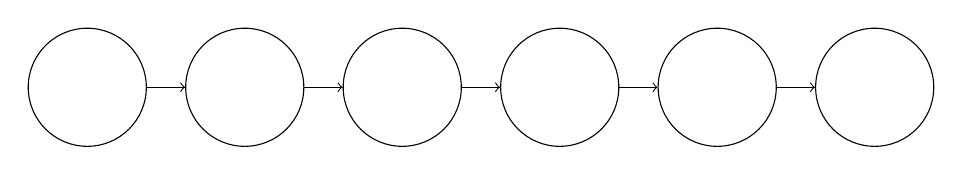
\begin{tikzpicture}[node distance=2cm, every node/.style={draw, circle, minimum size=1.5cm}]
    \node (sunny1) {\Sun};
    \node[right of=sunny1] (sunny2) {\HalfSun};
    \node[right of=sunny2] (partlycloudy) {\SunCloud};
    \node[right of=partlycloudy] (cloudy) {\Cloud};
    \node[right of=cloudy] (rainy) {\RainCloud};
    \node[right of=rainy] (sunny3) {\Sun};
    
    % Arrows
    \draw[->] (sunny1) -- (sunny2);
    \draw[->] (sunny2) -- (partlycloudy);
    \draw[->] (partlycloudy) -- (cloudy);
    \draw[->] (cloudy) -- (rainy);
    \draw[->] (rainy) -- (sunny3);
\end{tikzpicture}
    \end{center}
    {\footnotesize How could we model this?}
    \note{As we have seen before, we need more complicated models to understand more complicated relationships between variables. Now consider the following system: how do you describe a system like weather, where each event is dependent on the previous event? In the case of weather, we intuitively know that you're considerably more likely to have rain after a cloudy day than a sunny day, but the chance of having rain is going to decrease after several repeated days of heavy rain. In such a case, how do we describe this scenario?}
\end{frame}

\begin{frame}
    \frametitle{Markov Models}
    \begin{figure}[H]
        \centering
        \includegraphics[height=6cm]{images/weathermarkov.png}
    \end{figure}
    {\footnotesize Source: https://www.statology.org/markov-chains-demystified-from-weather-predictions-to-googles-pagerank/.}
    \note{The answer, of course, is using a statistical model known as a Markov Chain. These systems describe the relationship between several states and how the transition between each state carries distinct probabilities in scenarios based on random (or "Stochastic") behavior. All Markov chains can be said to consist of two fundamental components: states and outcomes. A state is the individual context within the Markov chain that you transition between, and outcomes are what we actually observe to happen as the result of the Markov chain's output. In the case of weather, the states and outputs are tied: we visually see that it's sunny outside, and the state of being sunny affects the chance of going to the next state. This distinction is important, as for every state, there is a set of probabilities of going to the next state (known as its transition probabilities) and producing the next output (known as its output probabilities).}
\end{frame}

\begin{frame}
    \frametitle{Core Question and Purpose}
    {\Large How complicated can we make a Markov model before we cannot accurately reverse-engineer it/predict its future behavior?}
    \begin{itemize}
        \item Many heavily researched strategies of reverse engineering stochastic models
        \item Not as much insight into how memory relates the effectiveness of reverse-engineering
    \end{itemize}
    \note{Of course, these systems can get quite complicated, and in reality, all we can actually observe is just the series of outputs. Everywhere in the real world, we see the effects of these "hidden" Markov chains playing out, and to model all sorts of behavior, from weather patterns to the spread of cancer cells, we need to be able to develop efficient systems to effectively guess what is going on under the surface for a Markov chain.}
\end{frame}

\section{Methods}
\begin{frame}
    \frametitle{Markov Model/Coin Systems}
    \begin{center}
    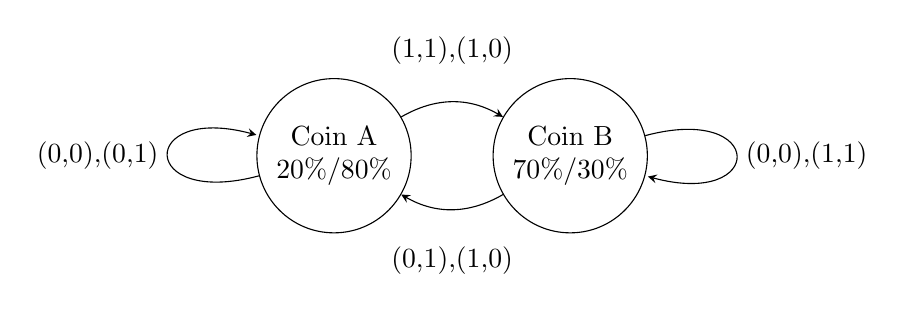
\begin{tikzpicture}[->, >=stealth, node distance=3cm, auto, scale=1, transform shape]

    % Define states
    \node[state, align=center] (A) {Coin A\\20\%/80\%};
    \node[state, right of=A, align=center] (B) {Coin B\\70\%/30\%};

    % Transitions
    \path   (A) edge [loop left]  node              {(0,0),(0,1)} (A)
                edge [bend left]  node[yshift=1em]  {(1,1),(1,0)} (B)
            (B) edge [loop right] node              {(0,0),(1,1)} (B)
                edge [bend left]  node[yshift=-1em] {(0,1),(1,0)} (A);

\end{tikzpicture}
    \end{center}
    \note{In this case, we're using a very simple example for using a Markov chain: modeling a system of coins or dice. Imagine we took a bunch of dice, which each have a distinct and uneven set of probabilities of producing their outputs, and wrote a series of rules dictating how we go from die to die given a series of outputs. Thinking back to our weather example, we know that the weather two days ago is very heavily involved in predicting the weather of tomorrow, but the weather of fifty years in the past will have little to no effect on the present weather other than in having effected the events that affect the current weather in a chain. As such, Markov chains can be said to have a certain "memory depth," or a number of outputs back at which we can look to better understand the behavior of the chain. In this case, we've defined a system that has a size of 2, so two coins and two outputs, and a memory depth of 2, meaning that the transition between each coin is based on the past two outputs.}
\end{frame}

\begin{frame}
    \frametitle{Complexity and Variance}
    Complexity
    \begin{equation}
        c = nvm^2
    \end{equation}

    Variance ($v$)
    \begin{equation}
        v = \sum_{i=1}^{n} \sum_{j=1}^{n} |p_{i,j} - \mu|, \mu = \frac{1}{n}
    \end{equation}
\end{frame}

\begin{frame}
    \frametitle{Error}
    Error
    \begin{equation}
    E(I,O) = \sum_{i=1}^{n} \sum_{j=1}^{n} |P_{I_{i,j}} - P_{O_{i,j}}|,
    \end{equation}
    \begin{itemize}
    \item The sum of the absolute differences for all probabilities across the distributions for all states on both systems.
    \end{itemize}
\end{frame}

\begin{frame}
    \frametitle{Core Pipeline}
    \begin{center}
    \resizebox{0.8\textwidth}{!}{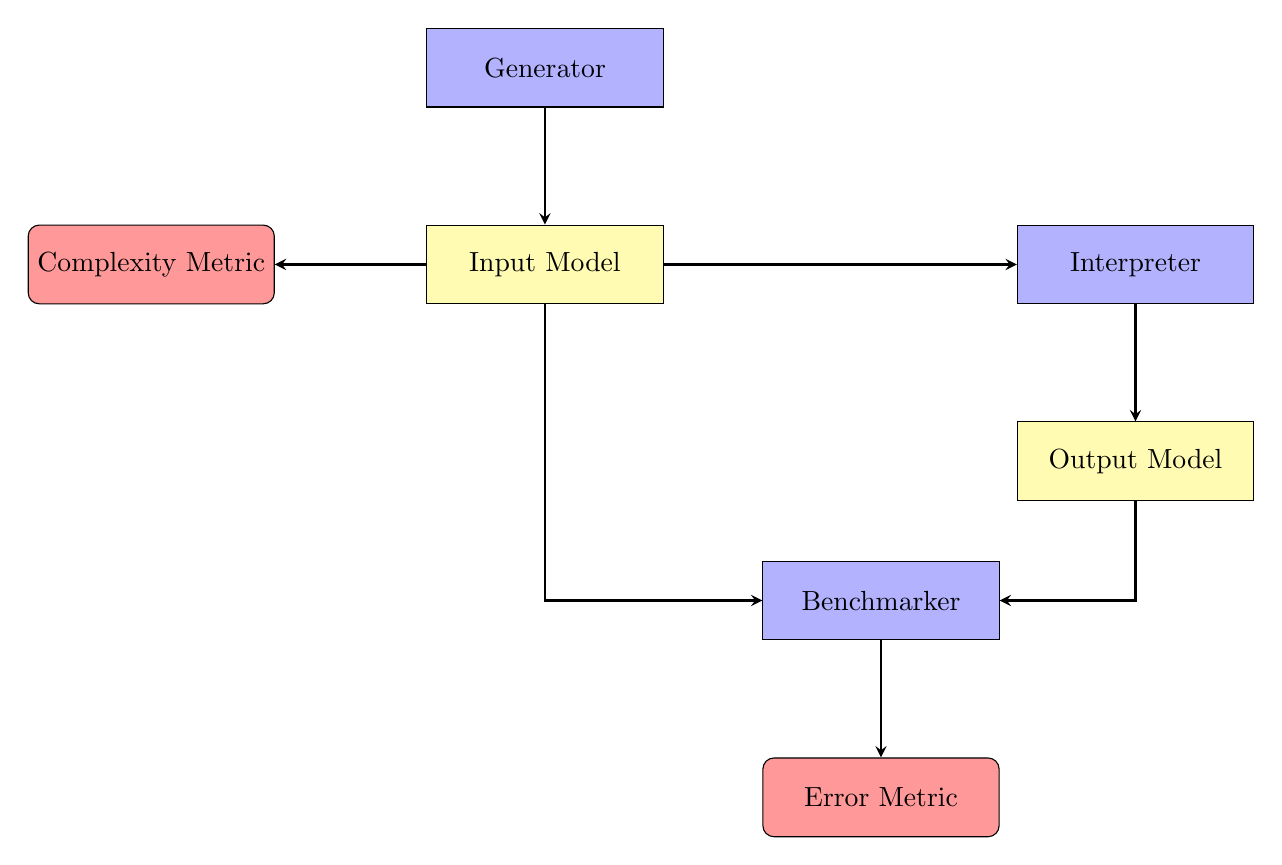
\begin{tikzpicture}[node distance=2.5cm]

    % Nodes
    \node (generator) [process, fill=blue!30] {Generator};
    \node (inputmodel) [process, below of=generator, fill=yellow!30] {Input Model};
    \node (interpreter) [process, right of=inputmodel, xshift=5cm, fill=blue!30] {Interpreter};
    \node (outputmodel) [process, below of=interpreter, fill=yellow!30] {Output Model};
    \node (benchmarker) [process, below right of=inputmodel, xshift=2.5cm, yshift=-2.5cm, fill=blue!30] {Benchmarker};
    \node (error) [startstop, below of=benchmarker, fill=red!40] {Error Metric};
    \node (complexity) [startstop, left of=inputmodel, xshift=-2.5cm, fill=red!40] {Complexity Metric};

    % Arrows
    \draw [arrow] (generator) -- (inputmodel);
    \draw [arrow] (inputmodel) -- (interpreter);
    \draw [arrow] (interpreter) -- (outputmodel);
    \draw [arrow] (inputmodel) |- (benchmarker);
    \draw [arrow] (outputmodel) |- (benchmarker);
    \draw [arrow] (benchmarker) -- (error);
    \draw [arrow] (inputmodel) -- (complexity);

\end{tikzpicture}}
    \end{center}
    Interpreter: pre-informed of the transition rules and iterates over the data to calculate probability distributions for each state by building a histogram.
    \note{Our testing pipeline begins at the generator, which will randomly generate a coin system like shown in the previous slide known as the "Input Model." This is the true model, and we want to reverse-engineer this. From that model, we use its probabilities, memory depth, and size to calculate a complexity metric, and then we run the input model to produce a sequence of 10,000 outputs. This output data alongside some select information about the input model is passed into the interpreter to reverse-engineer the input model using several solving algorithms, and these output models are then compared against the input model in the benchmarker to produce an error metric. Lastly, we compare the complexiy metric and the error metric to unerstand our data trend.}
\end{frame}

\section{Results}

\begin{frame}
    \frametitle{Results}
    \begin{figure}[H]
        \centering
        \includegraphics[width=\textwidth]{images/graph-all.png}
    \end{figure}
    \note{These are our testing results for solving coins up to a memory depth of 4 and a size of 5 using just the Calix algorithm. In the graph, each memory depth has a distinct pattern of curling upwards as the models within that memory depth get more complicated, indicating that the error increases locally for each memory depth. This is likely best explained by understanding how the complexity is calculated. What is likely the greatest source of error within each memory depth is an increase in the size of the model. The complexity of a model is defined to increase linearly with the size of the model, and the error seems to increase quadratically or exponentially as this size increases.}
\end{frame}

\begin{frame}
    \frametitle{Results}
    \begin{figure}[H]
        \centering
        \includegraphics[width=0.45\textwidth]{images/graph-mem1.png}
        \includegraphics[width=0.45\textwidth]{images/graph-mem2.png}
        \includegraphics[width=0.45\textwidth]{images/graph-mem3.png}
        \includegraphics[width=0.45\textwidth]{images/graph-mem4.png}
    \end{figure}
    \note{Here, we've split the graphs so you can see that the trend appears to clearly be positive and direct, and possibly either linear or quadratic.}
\end{frame}

\begin{frame}
    \frametitle{Results (Memory 1)}
    \begin{figure}[H]
        \centering
        \includegraphics[width=0.49\textwidth]{images/graph-mem1.png}
        \includegraphics[width=0.49\textwidth]{images/graph-mem4.png}
    \end{figure}
    Slope at $m=1$ is about 3, slope at $m=4$ is about 1.2
\end{frame}

\section{Uncertainties}
\begin{frame}
    \frametitle{Uncertainties}
    \begin{itemize}
   \item Error measurements have inherent uncertainty, but should have limited influence due to the quantity of data
    \item Auto-generated data, and arbitrary quantities raise doubts over validity of results, these questions could be answered by researching with 'real' datasets
    \item Further tests over larger ranges of complexity are necessary to further validate our findings
        \end{itemize}
\end{frame}

\section{Conclusion}
\begin{frame}
    \frametitle{Conclusion}
    \begin{itemize}
   \item As expected, there is a positive/direct relationship between complexity and error.
    \item Model relationship cannot be determined due to our arbitrary quantities
    \item Memory influences the range of error for a given range of complexity
        \end{itemize}
\end{frame}

\section{Question/Answer}
\begin{frame}
    Questions!
\end{frame}

\begin{frame}
    \frametitle{Example Complexity and Variance}
    \begin{tikzpicture}

    % Transition Matrix (Left Side)
    \node (T) {$P = \begin{bmatrix} P_A \\ P_B \end{bmatrix} = 
    \begin{bmatrix} 0.2 & 0.8 \\ 0.7 & 0.3 \end{bmatrix}$};

    % Table (Right Side)
    \node (M) [right=2cm of T] {
        $T =$
        \begin{tabular}{c|c c}
            Sequence & $T_{A}$ & $T_{B}$ \\ 
            \hline\rule{0pt}{13pt}
            (0,0) & A & B \\
            (0,1) & A & A \\
            (1,0) & B & A \\
            (1,1) & B & B \\
        \end{tabular}
    };

\end{tikzpicture}
    \begin{itemize}
    \item $n=2$ (width/height of $P$) and $m=2$ (length of all sequences).
    \item As $n=2$, $\mu = \frac{1}{2} = 0.5$.
    \begin{itemize}
        \item $v = |0.2 - 0.5| + |0.8 - 0.5| + |0.7 - 0.5| + |0.3 - 0.5| = 1.0$
        \item $c = nvm^2 = (2)(1)(2)^2 = 8$
    \end{itemize}
    \end{itemize}
\end{frame}

\begin{frame}
\frametitle{Error Example}
\begin{center}
\begin{tikzpicture}

    % Transition Matrices
    \node (P1) {
        $P_1 = \begin{bmatrix} 0.2 & 0.8 \\ 0.7 & 0.3 \end{bmatrix}$
    };
    
    \node (P2) [right=3cm of P1] {
        $P_2 = \begin{bmatrix} 0.5 & 0.5 \\ 0.5 & 0.5 \end{bmatrix}$
    };
    
    % Absolute Difference Matrix
    \node (AbsDiff) [below=1.5cm of $(P1)!0.5!(P2)$] {
        $\left| P_1 - P_2 \right| = 
        \begin{bmatrix} 
        |0.2 - 0.5| & |0.8 - 0.5| \\ 
        |0.7 - 0.5| & |0.3 - 0.5| 
        \end{bmatrix} =
        \begin{bmatrix} 
        0.3 & 0.3 \\ 
        0.2 & 0.2 
        \end{bmatrix}$
    };

    % Summation Step
    \node (Sum) [below=1.5cm of AbsDiff] {
        $\sum \left| P_1 - P_2 \right| = 0.3 + 0.3 + 0.2 + 0.2 = \mathbf{1.0}$
    };

\end{tikzpicture}
\end{center}
\end{frame}

\begin{frame}
\frametitle{Interpreter}
$n=2, m=2$
\begin{center}
\begin{tikzpicture}

    % DATASET
    \node (Data) at (0, 2.5) {\textbf{Dataset:} \quad 0,1,0,0,1,0,1,1,0,0};

    % Grouped Sequences
    \node (Grouped) at (0, 1.5) {
        \begin{tikzpicture}
            \foreach \i/\numA/\numB in {0/0/1, 1/1/0, 2/0/0, 3/1/0, 4/1/1, 5/0/0} {
                % Draw the two-number box
                \draw (\i,0) rectangle (\i+1,0.5);
                
                % Place numbers inside
                \node at (\i+0.25, 0.25) {\numA};
                \node at (\i+0.75, 0.25) {\numB};
            }
        \end{tikzpicture}
    };

    % Using Columns for Better Slide Layout
    \begin{scope}[yshift=-1.5cm]
        \node (HistogramLabel) at (-3, 1.8) {\textbf{Histogram}};
        \node (ProbLabel) at (3, 1.8) {\textbf{Probability Distribution}};

        % Histogram Table
        \node (Histogram) at (-3, 0) {
            \begin{tabular}{c|c}
                Sequence & Count \\ 
                \hline
                (0,1) & 2 \\
                (1,0) & 2 \\
                (0,0) & 2 \\
                (1,1) & 1 \\
            \end{tabular}
        };

        % Probability Distribution Table
        \node (ProbDist) at (3, 0) {
            \begin{tabular}{c|c}
                Sequence & Probability \\ 
                \hline
                (0,1) & $2/7 \approx 0.286$ \\
                (1,0) & $2/7 \approx 0.286$ \\
                (0,0) & $2/7 \approx 0.286$ \\
                (1,1) & $1/7 \approx 0.143$ \\
            \end{tabular}
        };
    \end{scope}

\end{tikzpicture}

\end{center}
\end{frame}

\end{document}